%%%%%%%%%%%%%%%%%%%%%%%%
% DO NOT CHANGE HERE
%%%%%%%%%%%%%%%%%%%%%%%%
\documentclass[letter]{amsart}
\renewcommand{\thesubsection}{\Alph{subsection}}
\def\doubleunderline#1{\underline{\underline{#1}}}
\newcommand\tab[1][1cm]{\hspace*{#1}}
\usepackage{titlesec}
\usepackage{textcomp}
\titleformat{\subsection}[frame]
{\normalfont} {} {2pt} {\normalsize\bfseries\filright\thesubsection.\quad}
\usepackage[english]{babel}
\usepackage[utf8]{inputenc}
\usepackage{enumerate}
\usepackage{amsmath,amsfonts, amssymb}
\usepackage{graphicx}
\usepackage[table,xcdraw]{xcolor}
\usepackage{tikz}
\usetikzlibrary{positioning,shapes,arrows}
\usepackage[margin=1in]{geometry}
\titleformat {\section}
  {\normalfont \Large \bfseries \centering}{\thesection}{1em}{}
\usepackage{enumitem}
\usepackage{mathrsfs}
\usepackage{caption}
\usepackage{hyperref}
\usepackage{subcaption}
\usepackage{float}
\usepackage[fontsize=12pt]{scrextend}
\restylefloat{table}
\usepackage{mathtools}
\newcommand{\rr}{\mathbb{R}}
\newcommand{\nn}{\mathbb{N}}
\newcommand{\qq}{\mathbb{Q}}
\newcommand{\dd}{$D$ }
\newcommand{\intt}{int \text{ }}
\newcommand{\bd}{bd \text{ }}
\newcommand{\nbd}{nbd \text{ }}
\newcommand{\cl}{cl \text{ }}
\newcommand{\me}{\mathrm{e}}
\newcommand\mypound{\protect\scalebox{0.8}{\protect\raisebox{0.4ex}{\#}}}
\definecolor{UMassMaroon}{RGB}{136,28,28}
\setcounter{MaxMatrixCols}{20}

%%%%%%%%%%%%%%%%%
% CHANGE HERE
%%%%%%%%%%%%%%%%%
\newcommand{\StudentName}{Harold Thidemann, Adi Geva, Dhruvi Chauhan}

%%%%%%%%%%%%%%%%%%%%%%%%
% DO NOT CHANGE HERE
%%%%%%%%%%%%%%%%%%%%%%%%
\title[Math 552: Applications Of Scientific Computing $\mid$ Project ]{Math 552: Applications Of Scientific Computing\\Project}
\author[\StudentName]{\StudentName}

\begin{document}
\maketitle

%%%%%%%%%%%%%%%%%
% CHANGE HERE
%%%%%%%%%%%%%%%%%

% \section*{Abstract}

\section*{\textbf{TO DO LIST:}}
its under this!
\begin{itemize}
	\item All the pictures - DONE
		\subitem - All the fingerprints and them at different points in their processing
	\item Included the code verbatim at the end and add that as a note somewhere in the beginning
	\item further expand upon results
		\subitem - the 3 OG images, and there images post SVD and the images of their Fourier amplitude spectrum
	\item further expand upon methods
		\subitem - Explain the three different type of finger prints
		\subitem - Explain how the transforms for each type should be similar
		\subitem - Explain SVD and FFT with respect to our experiment
	\item make sure everything is in this document!
	\item Remove abstract - DONE
	\item Complexity analysis, either time or space dependent on what the paper talked about
	\item add a  proper citation to the paper \\
	\href{https://scholar.google.com/scholar?hl=en&as_sdt=0%2C22&q=FINGERPRINT+CLASSIFICATION+USING+A+HEXAGONAL+FAST+FOURIER+TRANSFORM&btnG=}{Link to get your cites here} \\
	\begin{verbatim}
	Fitz, A. P., \& Green, R. J. (1996). Fingerprint classification using 
	     a hexagonal fast Fourier transform. Pattern 
	     recognition, 29(10), 1587-1597.
	\end{verbatim}
\end{itemize}
%So, we need an abstract here if we have an abstract. If not then we could just have the introduction as the start.



\section*{Introduction}
Fast Fourier Transforms are central in collecting and analyzing data. Audio sequences, images, and videos are compressed and represented efficiently using FFT. Modern digital communication is built on this, making this one of the most important algorithms developed. One application of FFT is analyzing fingerprints. Fingerprints have patterns, such as loops, whorls and arches, which are unique to every individual and therefore make this a useful tool for identification in law enforcement and forensics. A fingerprint image can be compressed for more efficient processing, analyzed using Fourier transform, and then classified accordingly.

In such image processing, rectangular sampling is often used. However, researchers have found that in this application, hexagonal sampling of pixels is optimal. In hexagonal sapling, each pixel is surrounded by six other pixels that are equidistant from itself. This optimizes both data storage and computational cost.

In order to reduce computation, an image of a fingerprint is preprocessed and stored in a 256x256 matrix and translated into a hexagonal grid. The preprocessing method also includes smoothing ridges and removing noise in and around the ridges.

Patterns in a fingerprint are characterized by parallel and periodic lines. Fourier transform is a fitting tool in this application since FT allows to approximate different functions using trigonometric functions of increasing frequencies. Thus, finding Fourier transforms of different fingerprint images and analyzing their frequencies is indicative of the spatial orientation of the ridges in arches, whorls, and loops. After applying HFFT,  nearest-neighbor classification was implemented to see how accurately this method classifies fingerprints. Using a database consisting of 40 fingerprint images, the algorithm gave a classification rate of 85\%.

Since every person has a unique fingerprint, the Fourier transform of an image of their fingerprint will be unique as well. 


\section*{Methods}
Methods here.

\begin{minipage}[H]{0.33\textwidth}
    \centering
    
\includegraphics[width=0.95\textwidth]{fingerprintARCH.jpeg}
    \captionof{figure}{Arch}
\end{minipage}
\begin{minipage}[H]{0.33\textwidth}
    \centering
    
\includegraphics[width=0.95\textwidth]{fingerprintWHORL.jpeg}
    \captionof{figure}{Whorl}
\end{minipage}
\begin{minipage}[H]{0.33\textwidth}
    \centering
    
\includegraphics[width=0.95\textwidth]{fingerprintLOOP.jpeg}
    \captionof{figure}{Loop}
\end{minipage}

\begin{minipage}[H]{0.33\textwidth}
    \centering
    
\includegraphics[width=0.95\textwidth]{fingerprintARCH_svd.jpg}
    \captionof{figure}{Arch}
\end{minipage}
\begin{minipage}[H]{0.33\textwidth}
    \centering
    
\includegraphics[width=0.95\textwidth]{fingerprintWHORL_svd.jpg}
    \captionof{figure}{Whorl}
\end{minipage}
\begin{minipage}[H]{0.33\textwidth}
    \centering
    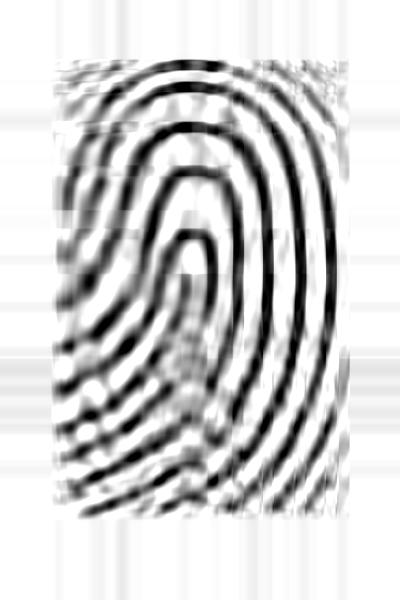
\includegraphics[width=0.95\textwidth]{fingerprintLOOP_svd.jpg}
    \captionof{figure}{Loop}
\end{minipage}

\newpage

\begin{minipage}[H]{0.33\textwidth}
    \centering
    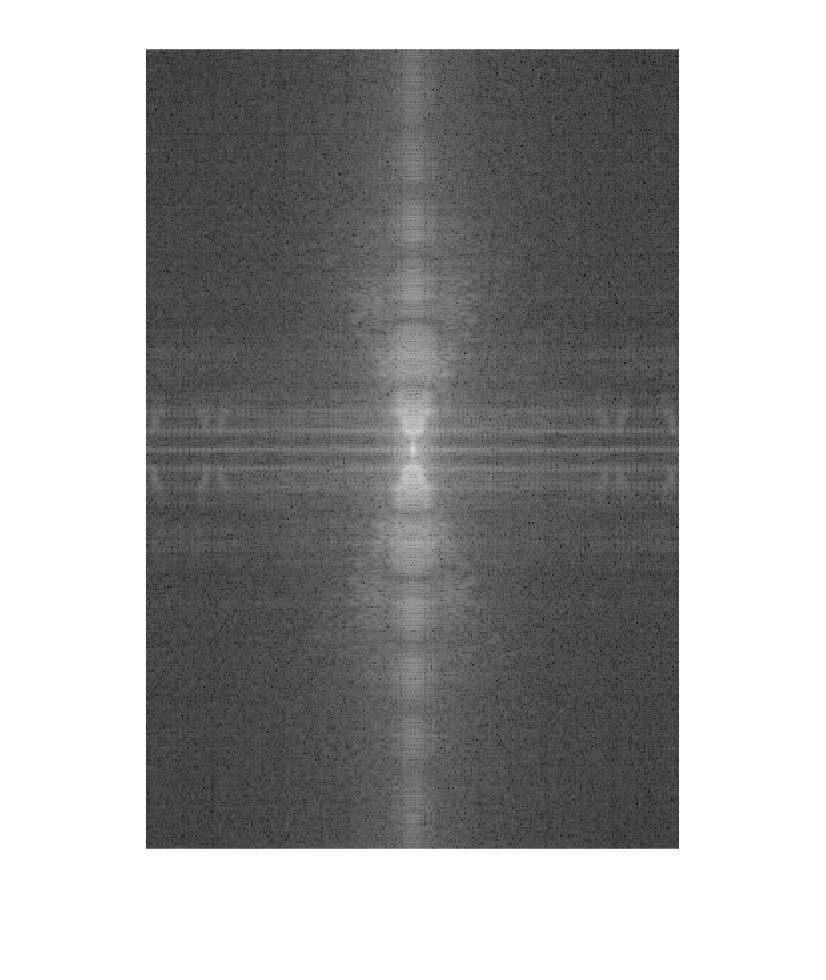
\includegraphics[width=0.95\textwidth]{fingerprintARCH_ft.jpg}
    \captionof{figure}{Arch}
\end{minipage}
\begin{minipage}[H]{0.33\textwidth}
    \centering
    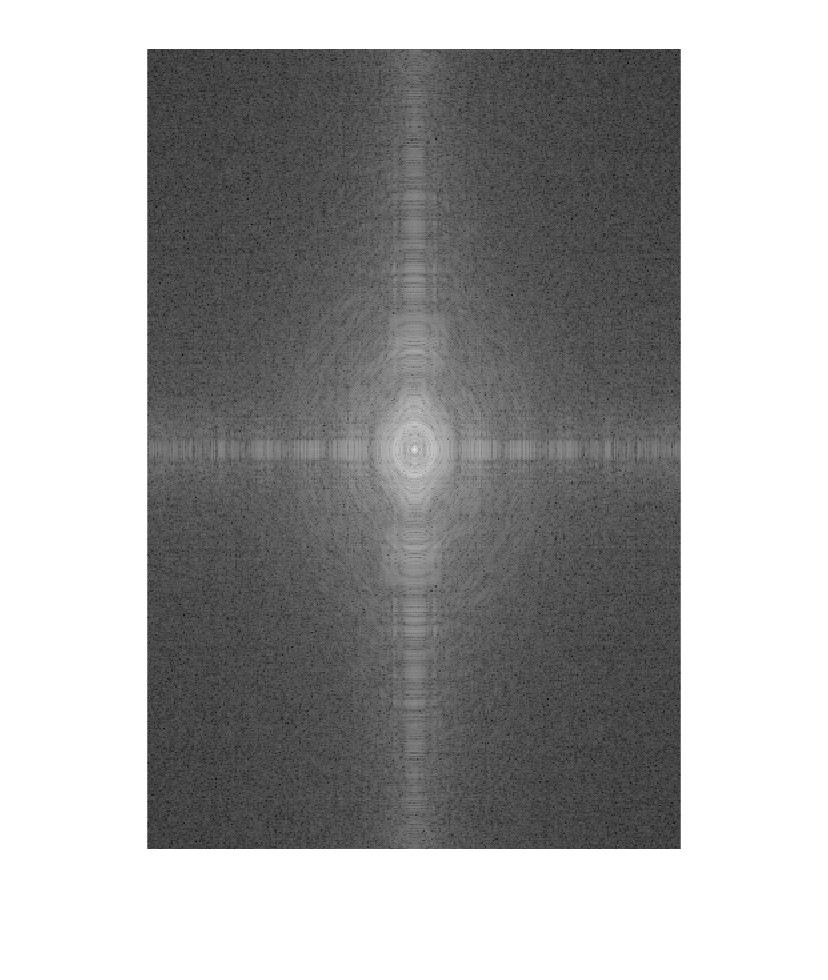
\includegraphics[width=0.95\textwidth]{fingerprintWHORL_ft.jpg}
    \captionof{figure}{Whorl}
\end{minipage}
\begin{minipage}[H]{0.33\textwidth}
    \centering
    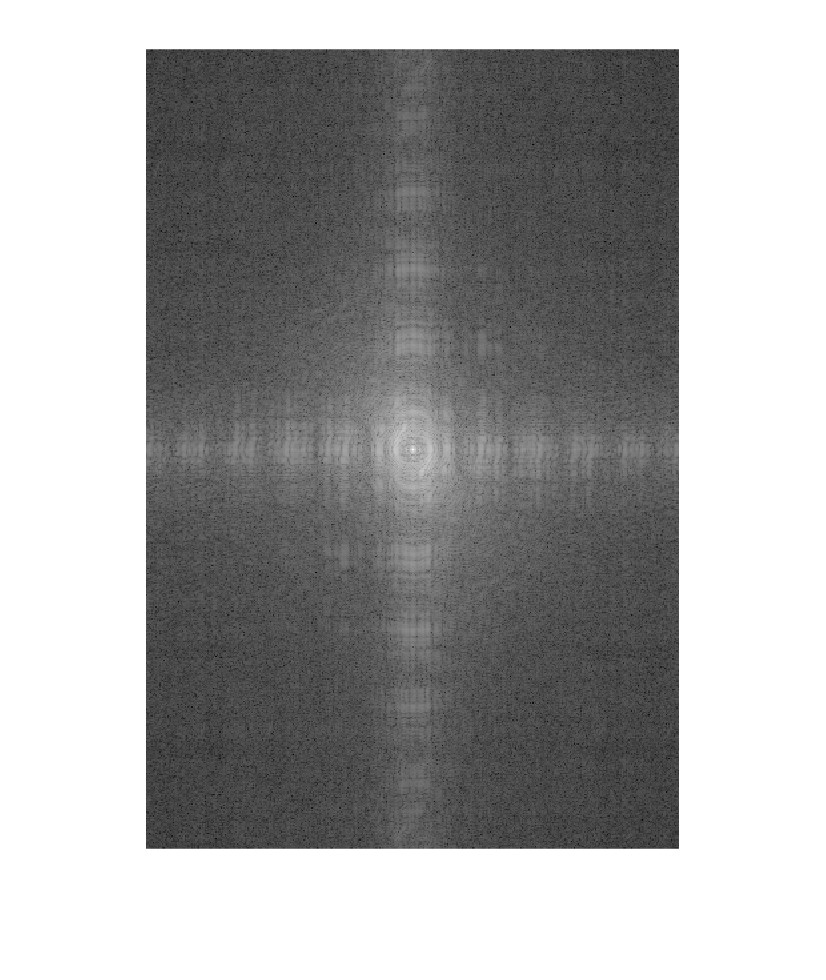
\includegraphics[width=0.95\textwidth]{fingerprintLOOP_ft.jpg}
    \captionof{figure}{Loop}
\end{minipage}


\section*{Results}
Results here.

In our project, we will modify the preprocessing step by performing image reduction using SVD on the input image. The original paper reduces the input image from 512x512 to 256x256 resolution by taking the average of four pixels and converting it to one pixel. We hope that by using SVD to reduce the image, we can preserve more valuable information from the original image while compressing it into lower resolution. To find the transform of the input image we will use MATLAB fft2 function. The function fft2 takes the Fast Fourier Transform of a 2 dimensional array which is the input image in this case.


We will start by creating a simple control case as our input which will be some scribbles drawn on Paint. This reduces the complexity of the problem by getting rid of the background noise issue that comes with fingerprint analysis. If we run the code twice on the same image we expect the output of the transform to be the same. Similarly, if we run the code in two images that are almost identical, we would expect the output of the transform to be very similar.
Time-permitting, we will also run the code on two images that are identical but rotated. If the code runs correctly, the transform should still be the same since it is the same drawing oriented differently. Ideally, the code will recognize that the image is identical and thus the patterns have the same frequency.


\newpage

\section*{Section 3}
Similarly, if a problem (or a subpart) ends up taking more than 1 page, please put (Continued) in the \verb!\section*! for that page.  You can also use \verb!\newpage! to choose where (in your work) the current page ends and where the next page begins.
\newpage

\section*{Section 3 (Continued)}
Like this.
\newpage

\section*{Example Proof}
\noindent\textbf{Want to Prove:} $x+y=x+z \ni x,y,z \in \mathcal{Z} \implies y=z$.\vspace{0.5em}\\
$\begin{aligned}
x+y &= x + z\\
(-x)+(x+y) &= (-x)+(x+z)\\
((-x)+x)+y&=((-x)+x)+z\\
0+y &= 0+z\\
y &= z \qed
\end{aligned}$
\text{ }\vspace{2em}\\
\textbf{\LaTeX\ Pro Tip}: They key to the \texttt{aligned} environment is to use the \& operator as what everything aligns to.  Note that, above, we always have it as \texttt{\&=}, meaning that each line has the \texttt{=} sign aligned to the same spot.  This makes the proof much easier to read.\vspace{1em}\\
\textbf{Math Pro Tip}: The $\qed$ symbol, called \href{https://en.wikipedia.org/wiki/Q.E.D.}{Q.E.D.}, is often used to signal the end of a proof.
\newpage

\section*{Example Math Work}
$\begin{aligned}
(1 + 2 + 3 + 4 + 5) \cdot 1000 &= (3+3+4+5) \cdot 1000\\
&= (6+4+5) \cdot 1000\\
&= (10+5) \cdot 1000\\
&= (15) \cdot 1000\\
1 + 2 + 3 + 4 + 5 &= \doubleunderline{15000}\\
\end{aligned}$
\text{ }\vspace{2em}\\
\textbf{\LaTeX\ Pro Tip}: Feel free to use the \verb!\doubleunderline! command to double-underline your final answer, which can make your work easier to read.
\newpage

\section*{Example Table}
\textbf{\LaTeX\ Pro Tip}: Use \href{https://tablesgenerator.com/}{tablesgenerator.com} to save \textit{a lot} of time when making tables.  You can even copy/paste from Excel or import a CSV!
\begin{table}[H]
\begin{tabular}{|c|c|c|c|c|}
\hline
\rowcolor[HTML]{333333} 
{\color[HTML]{FFFFFF} \textbf{Column 1}} &
  {\color[HTML]{FFFFFF} \textbf{Column 2}} &
  {\color[HTML]{FFFFFF} \textbf{Column 3}} &
  {\color[HTML]{FFFFFF} \textbf{Column 4}} &
  {\color[HTML]{FFFFFF} \textbf{Column 5}} \\ \hline
 &  &  &  &  \\ \hline
 &  &  &  &  \\ \hline
 &  &  &  &  \\ \hline
 &  &  &  &  \\ \hline
 &  &  &  &  \\ \hline
\end{tabular}
\caption{Table Caption Here}
\end{table}
\newpage

\section*{Using an Uploaded Photo}
\textbf{\LaTeX\ Pro Tip}: Avoid using underscores in file names to make your life easier.  \href{https://tex.stackexchange.com/questions/58689/how-to-use-an-underscore-in-a-filename}{There are ways around this} but it's likely easier to just rename a file.
\begin{figure}[H]
    \centering
    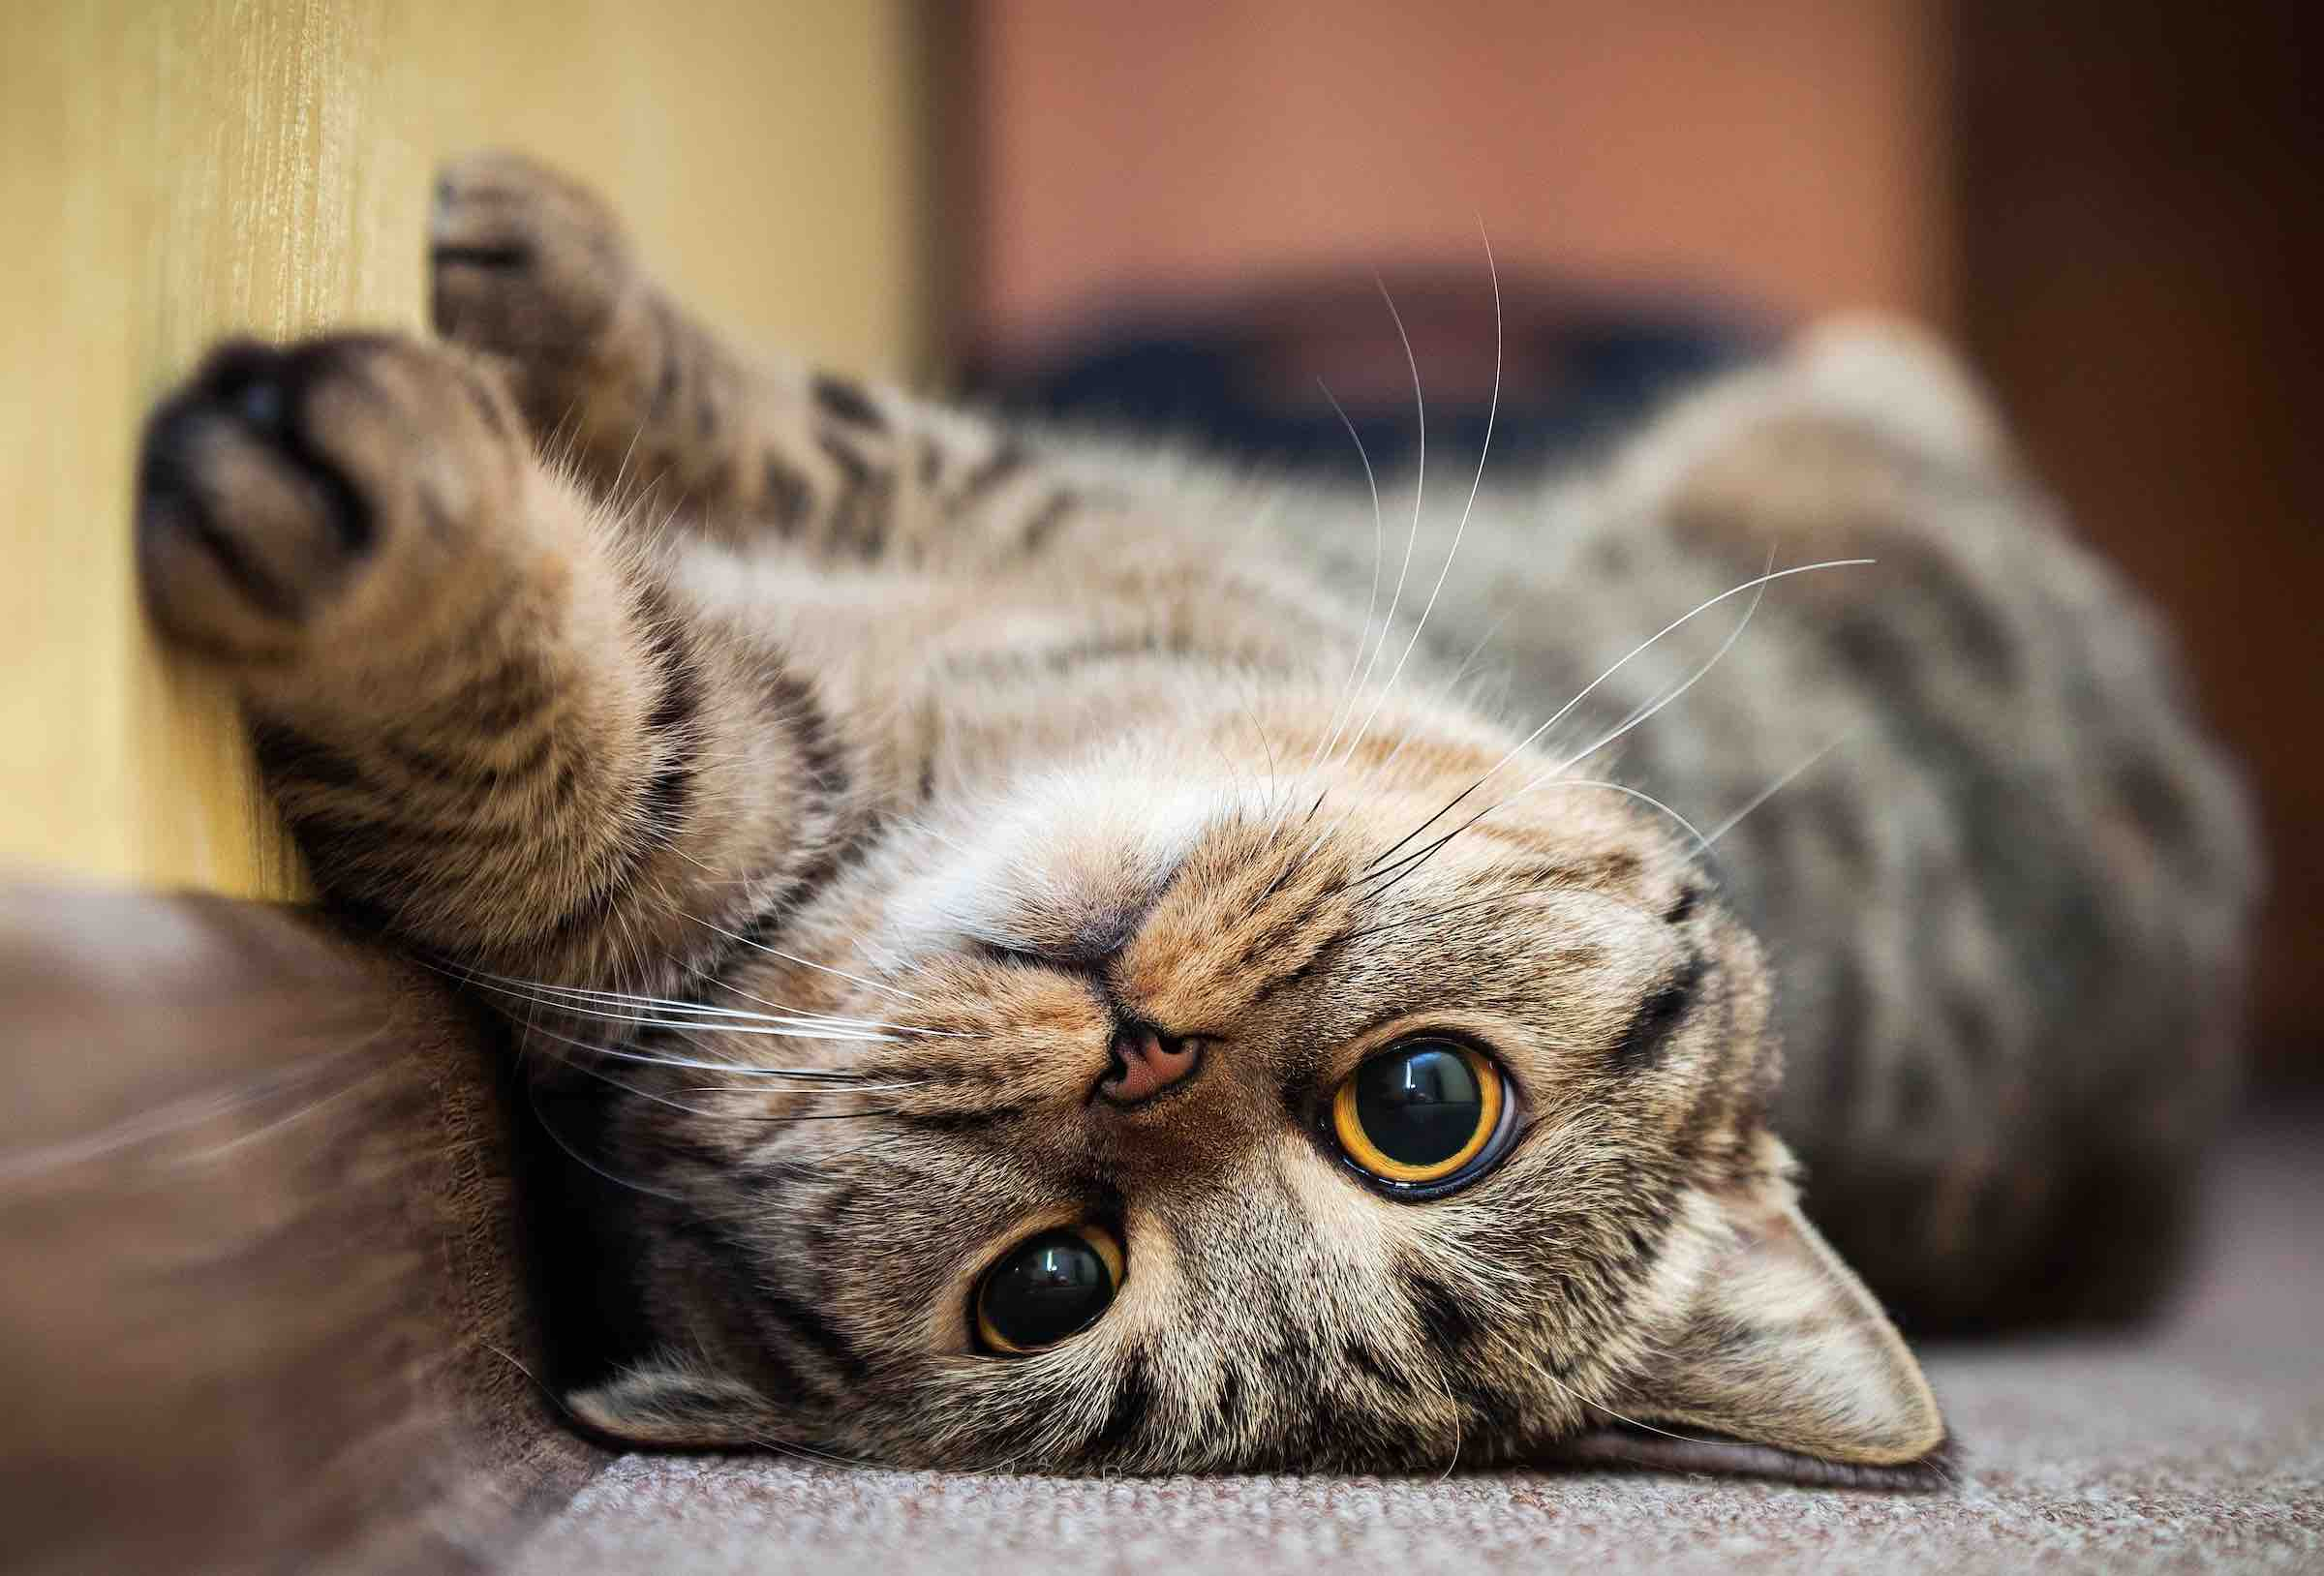
\includegraphics[width=0.5\textwidth]{cute-kitten.jpg}
    \caption{Example Image A}
\end{figure}
\newpage

\section*{Single Figure}
\textbf{\LaTeX\ Pro Tip}: To remove the image caption, comment out the \verb!\caption! line.
\begin{figure}[H]
    \centering
    \includegraphics[width=0.5\textwidth]{example-image-a}
    \caption{Example Image A}
\end{figure}
\newpage

\section*{Two Side-By-Side Figures}
\begin{minipage}[H]{0.5\textwidth}
    \centering
    \includegraphics[width=0.8\textwidth]{example-image-a}
    \captionof{figure}{Example Image A}
\end{minipage}
\begin{minipage}[H]{0.5\textwidth}
    \centering
    \includegraphics[width=0.8\textwidth]{example-image-b}
    \captionof{figure}{Example Image B}
\end{minipage}
\newpage

\section*{Three Side-By-Side Figures}
\begin{minipage}[H]{0.33\textwidth}
    \centering
    \includegraphics[width=0.95\textwidth]{example-image-a}
    \captionof{figure}{Example Image A}
\end{minipage}
\begin{minipage}[H]{0.33\textwidth}
    \centering
    \includegraphics[width=0.95\textwidth]{example-image-b}
    \captionof{figure}{Example Image B}
\end{minipage}
\begin{minipage}[H]{0.33\textwidth}
    \centering
    \includegraphics[width=0.95\textwidth]{example-image-c}
    \captionof{figure}{Example Image C}
\end{minipage}
\newpage

\section*{Side-By-Side Figure and Table}
\begin{minipage}[H]{0.5\textwidth}
    \centering
    \includegraphics[width=0.8\textwidth]{example-image-a}
    \captionof{figure}{Example Image A}
\end{minipage}
\begin{minipage}[H]{0.5\textwidth}
\resizebox{\textwidth}{!}{%
\begin{tabular}{|c|c|c|c|c|}
\hline
\rowcolor[HTML]{333333} 
{\color[HTML]{FFFFFF} \textbf{Column 1}} &
  {\color[HTML]{FFFFFF} \textbf{Column 2}} &
  {\color[HTML]{FFFFFF} \textbf{Column 3}} &
  {\color[HTML]{FFFFFF} \textbf{Column 4}} &
  {\color[HTML]{FFFFFF} \textbf{Column 5}} \\ \hline
 &  &  &  &  \\ \hline
 &  &  &  &  \\ \hline
 &  &  &  &  \\ \hline
 &  &  &  &  \\ \hline
 &  &  &  &  \\ \hline
\end{tabular}%
}
\captionof{table}{Table Caption}
\end{minipage}
\newpage

\end{document}